\documentclass[a4paper]{article}
\usepackage{amsfonts}
\usepackage{amsmath}
\usepackage{amssymb}
\usepackage{graphicx}

\newcommand{\dint}{\displaystyle\int}

\begin{document}

\noindent \large Auteur: Rob Willemsen \\
\noindent \large Studierichting: Informatica \\
\noindent \large Oefeningenreeks 5G nr. 10 \\

\medskip

\normalsize

Klein teken onderzoek: \\

$y = 0 \Rightarrow 0 = \dfrac{x^2 (1+x)}{1-x} \Rightarrow x = 0 $ en $ x = -1 $ \\

$f(x) = \dfrac{x^2+x^3}{1-x}$ \\

$f'(x) = \dfrac{(2x+3x^2)(1-x) + (x^2+x^3)}{(1-x)^2}$ \\

$= \dfrac{2x+3x^2-2x^2-3x^3+x^2+x^3}{(1-x)^2}$ \\

$= \dfrac{2x+2x^2-2x^3}{(1-x)^2} \Rightarrow x^2-x-1 = 0 $ \\

$\Delta = 1^2 - 4 \cdot 1 \cdot (-1) = 5$ \\

$x = \dfrac{-(-1) \pm \sqrt{5}}{2 \cdot 1} = \dfrac{1 \pm \sqrt{5}}{2}$ \\

$\dfrac{1 - \sqrt{5}}{2} \approx -0.618$ \\

$y^2 = \dfrac{(-0.618)^2 \cdot (1+(-0.618))}{1-(-0.618)} \approx 0.09 \Rightarrow y \approx 0.3 $ \\

\begin{figure}[h]
\centering
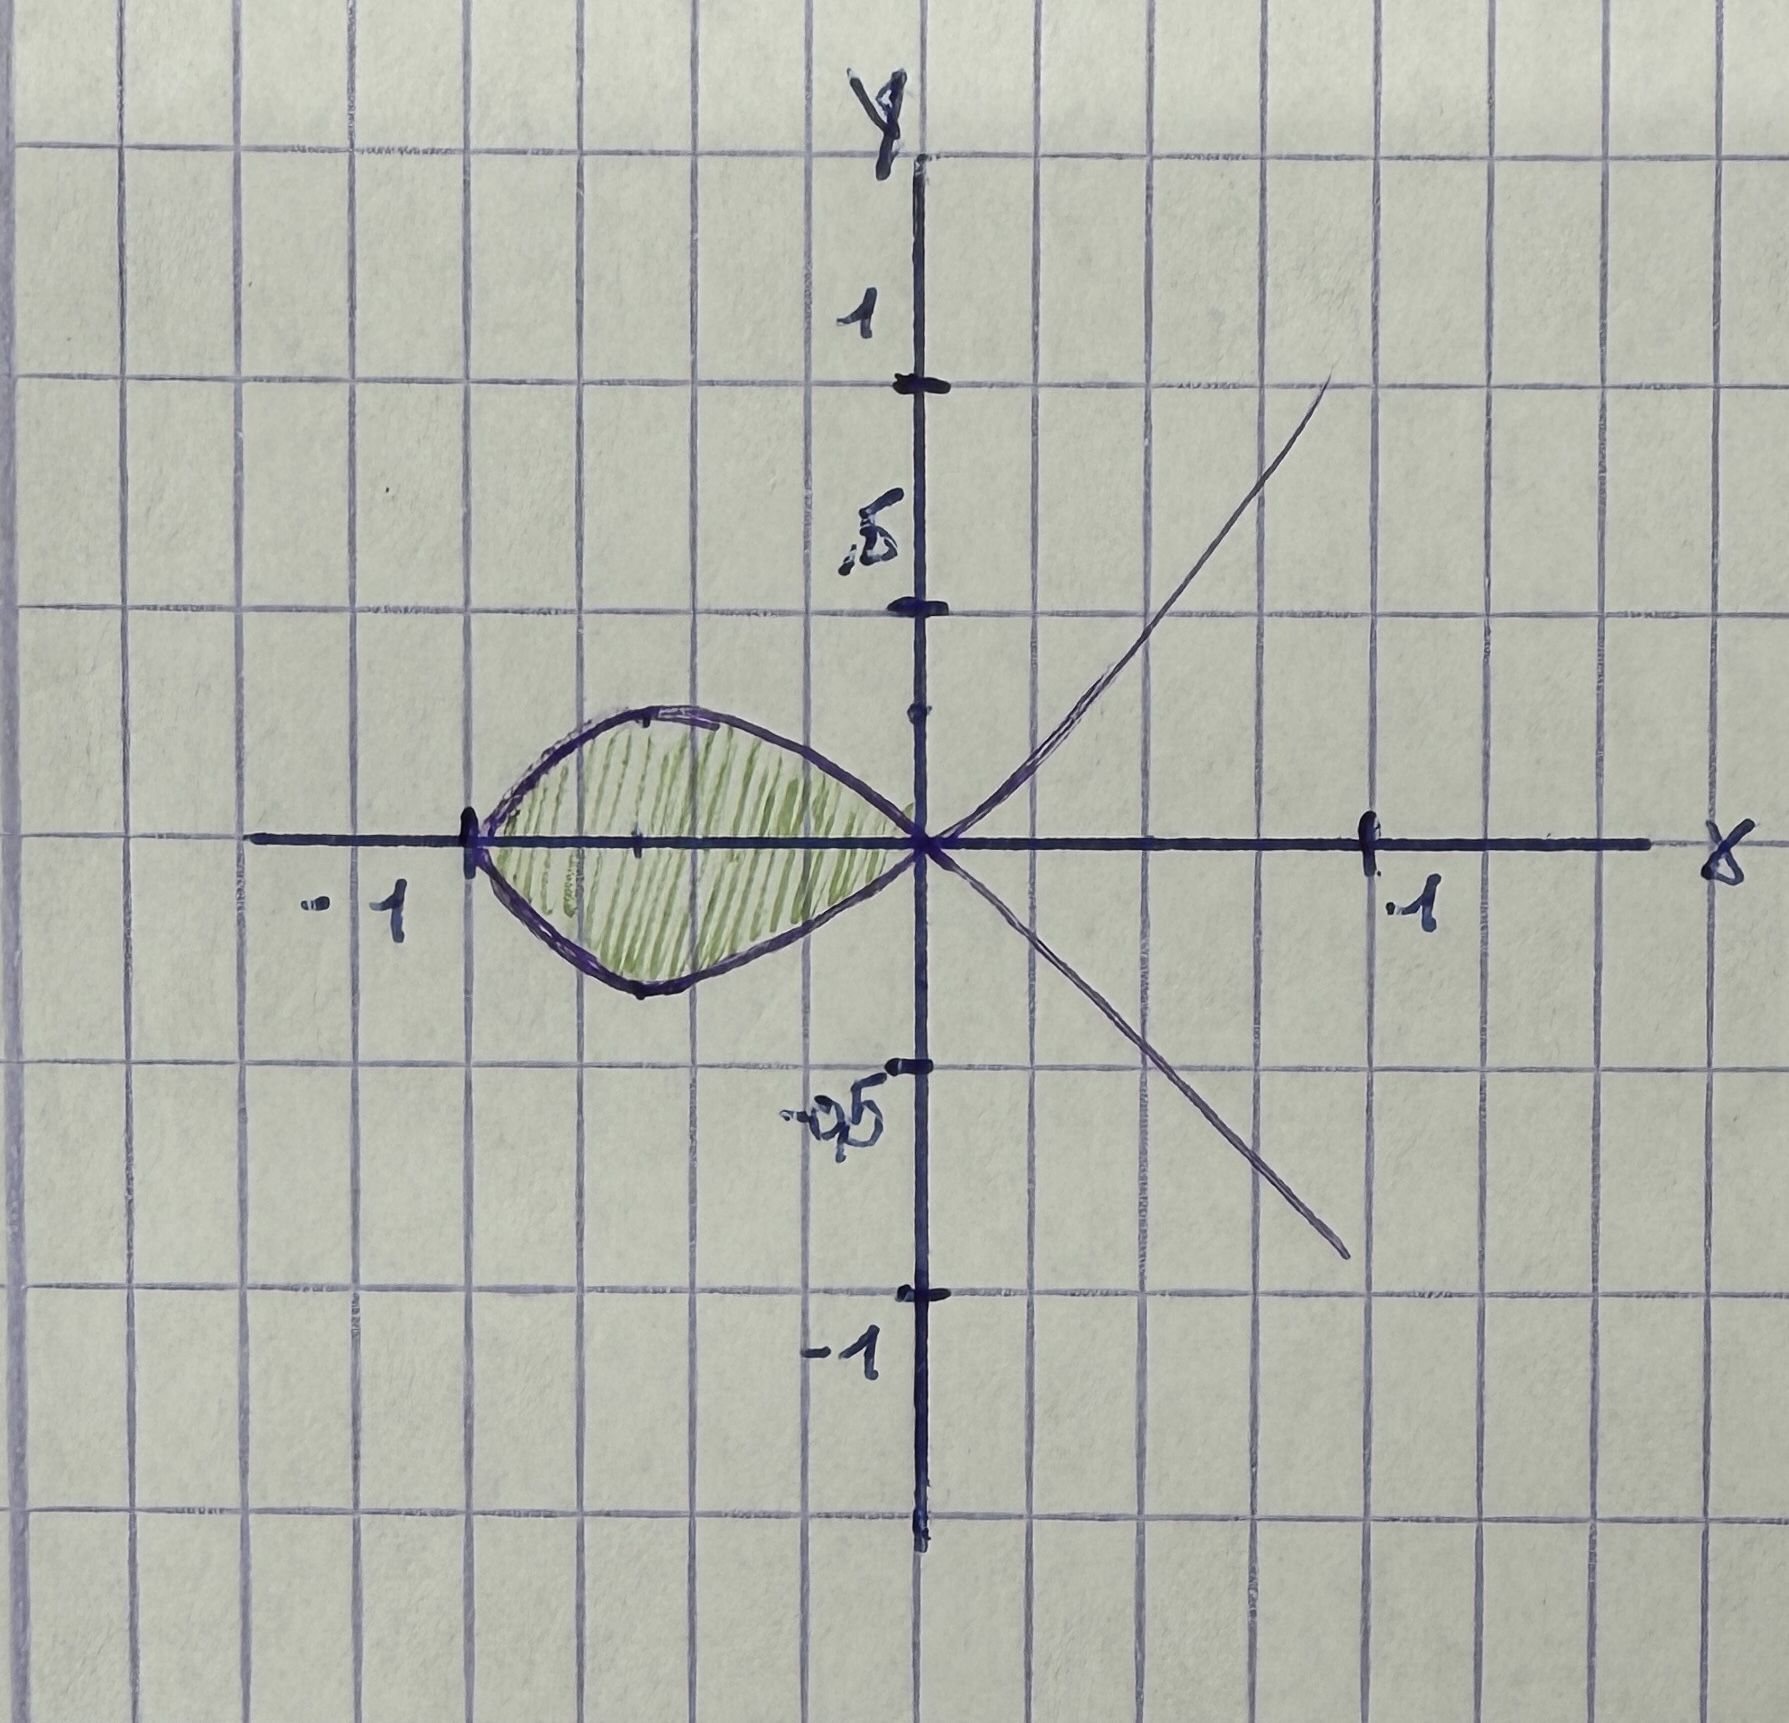
\includegraphics[width=0.5\linewidth]{5G-10-rob.willemsen.INF.png}
\end{figure}

Berekening:

$V = \pi \dint_{-1}^{0} \dfrac{x^2(1+x)}{1-x} dx$ \\

$t=1-x \Rightarrow dt = -dx \Rightarrow -dt = dx$ \\

$=\pi \dint_{2}^{1} \dfrac{(1-t)^2 \cdot (1 + (1-t))}{t} (-dt)$ \\

$=\pi \dint_{1}^{2} \dfrac{(t^2-2t+1) \cdot (2-t)}{t} dt$ \\

$=\pi \dint_{1}^{2} \dfrac{(-t^3+4t^2-5t+2)}{t} dt$ \\

$=\pi \dint_{1}^{2} (-t^2+4t-5+\dfrac{2}{t}) dt$ \\

$=\pi \left[ -\dfrac{t^3}{3} + 2t^2 - 5t + 2 \ln(t) \right]_{1}^{2}$ \\

$=\pi \left( -\dfrac{8}{3} + 8 - 10 + 2 \ln(2) + \dfrac{1}{3} - 2 + 5 + 2 \ln|1| \right)$ \\

$=\pi \left(2 \ln|2| - \dfrac{14}{3} + \dfrac{10}{3} \right)$ \\

$=\pi \left(2 \ln|2| - \dfrac{4}{3} \right)$ \\

\begin{thebibliography}{999}
%\bibitem{a} Referentie
\end{thebibliography}
\end{document}